\documentclass[11pt,a4paper]{article}
\usepackage[margin=1in]{geometry}
\usepackage[T1]{fontenc}
\usepackage[utf8]{inputenc}
\usepackage{lmodern}
\usepackage{amsmath,amssymb}
\usepackage{booktabs}
\usepackage{tabularx}
\usepackage{graphicx}
\usepackage{tikz}
\usepackage{hyperref}
\usepackage{setspace}
\usepackage{enumitem}
\usepackage{array}
\usepackage{caption}
\usepackage{url}
\setstretch{1.0}
\hypersetup{colorlinks=true,linkcolor=black,citecolor=black,urlcolor=blue}
\setlength{\parskip}{0.45em}
\setlength{\parindent}{1.2em}
\setlist[itemize]{leftmargin=1.4em,itemsep=0.15em}
\setlist[enumerate]{leftmargin=1.4em,itemsep=0.15em}

\title{Equal-Exposure Depth and Held-Out Tagalog Bits-per-Byte on WikiText-TL-39}
\author{Paul Pajo\\
Independent Researcher\\
\texttt{paulamerigo.pajojr@benilde.edu.ph}}
\date{16 August 2026}

\begin{document}
\maketitle

\begin{abstract}
Does increasing decoder depth from 8 to 20 reduce held-out Tagalog bits-per-byte (BPB) when every depth sees the same model-visible token budget on WikiText-TL-39? This question was preregistered as AsPredicted \#306780 before confirmatory BPB existed. The study uses one public Parquet mirror of Cruz and Cheng's 2019 Tagalog Wikipedia language-modeling corpus, a train-only 32{,}768-merge byte-pair encoding (BPE) tokenizer, sequence length $T=2048$, and Karpathy's nanochat base trainer pinned at commit \texttt{92d63d4}. Original 2019 train, validation, and test files were not recovered. Splits were rebuilt by exact UTF-8 hash on reconstructed articles (label \texttt{reconstructed\_article\_70\_15\_15}). The common budget is $D_{3x}=3\times T_{\mathrm{train}}$, implemented as $N=294$ steps at batch $B=65{,}536$ tokens ($D_{\mathrm{actual}}=19{,}267{,}584$). Primary outcome is full-split validation BPB after the final checkpoint. Depth 20 is the exact numerical minimum ($1.172248$), $0.006887$ below depth 8. With one seed, gaps below $0.01$ BPB are not interpreted as a ranking. The series is not a clean fall-then-flatten: validation BPB rises from 8 to 16, then dips at 20, while the train--validation gap widens from 8 to 16. One test BPB ($1.164768$) was read after validation-only selection. All four trained models beat an untrained same-depth control and a train-fitted UTF-8 byte unigram. The contribution is a locked equal-exposure measurement on this corpus, not a claim that deeper models are always better, and not a chat, classification, or English CORE result.
\end{abstract}

\noindent\textbf{Keywords:} Tagalog language modeling; bits-per-byte; transformer depth; equal-exposure scaling; WikiText-TL-39; preregistration; low-resource NLP; nanochat; BPE; confirmatory evaluation.

\noindent\textbf{arXiv categories:} cs.CL, cs.LG.

\noindent\textbf{Code and weights:} study repository \texttt{nanochat-filipino}; model card and seed-0 checkpoints at \url{https://huggingface.co/pageman/nanochat-filipino-p1-fixed-d20-3x}. Registration: \url{https://aspredicted.org/6r6v4v.pdf}.

\section{Introduction}
\label{sec:intro}

Tagalog language modeling still sits on a small public Wikipedia-style corpus rather than on a web-scale mix. Cruz and Cheng introduced WikiText-TL-39 as a Tagalog analogue of WikiText, with about 39 million training tokens in the 2019 release~\cite{cruz2019eval}. Later Filipino pretraining work moved to larger mixed corpora and encoder models~\cite{cruz2022tlunified}. Those later resources answer a different question. They do not say what happens to held-out BPB when a decoder-only Transformer is made deeper while the number of model-visible tokens is held fixed on the original WikiText-TL-39 package.

Scaling studies in English treat depth, width, data, and compute as jointly chosen~\cite{kaplan2020scaling,hoffmann2022chinchilla,muennighoff2023dataconstrained}. A common operational shortcut is to let a larger model see more tokens, or to train to a native parameter-to-data ratio. That shortcut confounds depth with exposure. The present study removes that confound for one corpus and one trainer. Every confirmatory depth sees the same $D_{3x}=3\times T_{\mathrm{train}}$ budget. The trainer is nanochat, a small public decoder stack with an official depth dial~\cite{karpathy2026nanochat}. The metric is bits per UTF-8 byte, which compares models across tokenizers~\cite{shannon1951prediction,brown2020gpt3,melis2018eval}.

The original 2019 split files were not recoverable from the public Hugging Face Parquet mirror or from the historical S3 zip. That fact is part of the result, not a silent cleanup. The study therefore uses a documented article-hash 70/15/15 reconstruction and prints that label on every table.

The confirmatory question, filed before confirmatory BPB existed, is:

\begin{quote}
Does increasing nanochat depth from 8 to 20 reduce held-out Tagalog BPB when every depth sees $D_{3x}=3\times T_{\mathrm{train}}$ on WikiText-TL-39?
\end{quote}

The registered prediction was that validation BPB would fall then flatten, or that the train--validation gap would widen. The filing stated that the study would not claim that deeper is always better, and that it is not a CORE, chat, or classification test~\cite{aspredicted306780}.

This paper contributes four things.

\begin{enumerate}
\item A preregistered equal-exposure depth grid $\{8,12,16,20\}$ on WikiText-TL-39, with $T$, tokenizer, split, and token budget frozen before confirmatory outcomes.
\item A recoverable data path: Parquet hash, LF-only canonical text, reconstructed-article split, train-only 32{,}768 BPE, and isolated test text.
\item A one-test-touch evaluation: full validation BPB on every depth, exact-minimum selection of $D^{\ast}$, then one test BPB on $D^{\ast}$ only.
\item A negative main claim at the registered practical threshold: with one seed, the $0.006887$ BPB gap between depth 20 and depth 8 is below $0.01$ and is not a depth ranking.
\end{enumerate}

The paper follows the close-out checklist for AsPredicted \#306780. It does not amend that registration.

\section{Related work}
\label{sec:related}

\subsection{Filipino and Tagalog language resources}
Cruz and Cheng constructed WikiText-TL-39 by scraping Tagalog Wikipedia with a WikiText-like pipeline and released it as a language-modeling benchmark~\cite{cruz2019eval}. The same line of work later built TLUnified and RoBERTa-Tagalog models for classification~\cite{cruz2022tlunified} and studied transfer under labeled-data scarcity~\cite{cruz2020fakenews}. Those papers treat Filipino as a low-resource language in the practical sense: public text exists, but clean long-context language-modeling splits and decoder scaling measurements remain thin.

Work from Cheng's group in 2023--2026 stayed close to concrete Philippine tasks rather than to English leaderboard transfer. Examples include semantic grammar-error correction~\cite{espiritu2023balarila}, automatic Filipino WordNet induction~\cite{velasco2023wordnet}, telecommunications named-entity recognition~\cite{chan2023ner}, Chavacano language identification~\cite{vicente2024vardial}, 19th-century authorship attribution~\cite{espiritu2024aa}, formality style transfer~\cite{loquinte2024formality}, synthetic-data detection of AI-generated Filipino news~\cite{ong2025aigenerated}, sarcasm detection~\cite{marcellana2025sarcasm}, sparse-autoencoder analysis of code correctness~\cite{tahimic2025sae}, and a Chavacano machine-translation corpus~\cite{vicente2026chavacano}. The house style is consistent: name the language and the missing resource, build or adapt a dataset, report exact scores, and keep the claim inside the constructed task. The present paper uses that style on a language-modeling question that those later papers do not answer.

Southeast Asian multilingual surveys and encoder models provide broader context~\cite{conneau2020xlmr,cahyawijaya2023nusacrowd} but mix languages and objectives. They are not a substitute for a locked Tagalog Wikipedia BPB measurement.

\subsection{Language-modeling evaluation}
WikiText established a clean Wikipedia language-modeling setup in English~\cite{merity2017pointer}. BPB and related byte-normalized losses remain the fair comparison when vocabularies differ~\cite{shannon1951prediction,graves2013generating,melis2018eval,brown2020gpt3,gao2020pile}. This study uses nanochat's official \texttt{evaluate\_bpb}: mean token negative log-likelihood divided by $\ln 2$ times mean UTF-8 bytes per token, with special tokens excluded.

\subsection{Scaling, depth, and data constraints}
Kaplan et al.\ described power-law loss versus compute, data, and parameters~\cite{kaplan2020scaling,henighan2020scaling}. Hoffmann et al.\ argued that many large models were undertrained relative to their parameter count~\cite{hoffmann2022chinchilla}. Muennighoff et al.\ studied repeated epochs when unique data are scarce~\cite{muennighoff2023dataconstrained}. Pythia documented checkpointed decoder scaling under a shared recipe~\cite{biderman2023pythia}. Depth-versus-width analyses show that extra layers are not a free improvement once data and compute are fixed~\cite{levine2020depth,press2020reordering,tay2022scale}. The present grid is closer to a data-constrained equal-exposure test than to a Chinchilla-optimal sweep: $R_d=D_{3x}/P_{\mathrm{scaling}}$ falls from $0.46$ at depth 8 to $0.044$ at depth 20.

\subsection{Tokenization}
BPE remains the default subword method for this trainer~\cite{sennrich2016bpe,kudo2018sentencepiece}. GPT-2's English BPE is a known baseline, not a selection rule~\cite{radford2019gpt2}. Fertility on this validation split is descriptive only (Tagalog 32{,}768 BPE $\approx 4.53$ bytes/token versus GPT-2 $\approx 2.76$).

\subsection{Preregistration and confirmatory practice}
Preregistration reduces undisclosed flexibility in analysis~\cite{simmons2011falsepositive,wagenmakers2012confirmatory,nosek2018prereg,munafo2017manifesto}. AsPredicted \#306780 locked the question, depths, corpus, tokenizer size, sequence length, primary metric, baselines, exclusions, and the one-test-touch rule before confirmatory BPB existed~\cite{aspredicted306780}. Execution clarifications defined $T_{\mathrm{train}}$, $P_{\mathrm{scaling}}$, the final-checkpoint rule, and unigram smoothing without adding a new hypothesis.

\section{Glossary}
\label{sec:glossary}

\begin{description}[style=nextline,leftmargin=1.25em]
\item[BPB] Bits per byte. Primary unit. Lower is better.
\item[\texttt{val\_bpb\_full}] Official full-split validation BPB after the final checkpoint. Primary dependent variable.
\item[\texttt{test\_bpb}] The same formula on the isolated test split. Secondary. Read once, after $D^{\ast}$ is sealed.
\item[$T_{\mathrm{train}}$] Sum of BPE token lengths over frozen canonical train articles. No BOS, no packing, no crop. Here $6{,}401{,}013$.
\item[$D_{3x}$] Registered exposure target $3\times T_{\mathrm{train}}=19{,}203{,}039$ tokens.
\item[$D_{\mathrm{actual}}$] Tokens seen in training: $N\times B=294\times 65{,}536=19{,}267{,}584$ ($+0.336\%$ overshoot from integer steps).
\item[$P_{\mathrm{total}}$] All nanochat parameters, including value embeddings.
\item[$P_{\mathrm{scaling}}$] Transformer matrices plus language-model head. Used for $R_d=D_{3x}/P_{\mathrm{scaling}}$.
\item[$D^{\ast}$] Depth with the exact lowest final \texttt{val\_bpb\_full}. Here 20.
\item[$T$] Context length in tokens. Frozen at 2048.
\item[BPE] Byte-pair encoding. One 32{,}768-merge tokenizer, train documents only.
\item[BOS-bestfit] nanochat packing that prefixes BOS and packs documents into length-$T$ blocks, cropping leftovers.
\item[CORE] English multiple-choice suite. Excluded from this study.
\item[SFT] Supervised fine-tuning for chat. Excluded.
\item[ClimbMix] nanochat's default pretraining mix. Never downloaded.
\item[LF-only canonical] Source text with newline normalization only. No Moses detokenization.
\end{description}

\section{Methods}
\label{sec:methods}

\subsection{Registration and authority}
AsPredicted \#306780 is the governing record (PDF SHA-256 \texttt{a34f119d\ldots cc5ca})~\cite{aspredicted306780}. A pre-Gate-A note defined computations already named by the registration. Manifests and deviation cards document execution. They do not revise the question. Exploratory items (extra seeds, $D_{1x}$ pilots, gzip, document bootstrap, samples) stay outside the primary table.

\subsection{Corpus and canonical text}
Source: \texttt{linkanjarad/Wikitext-TL39}, file \texttt{data/train.parquet}, SHA-256 \texttt{706d7064\ldots 3caf9}, $1{,}524{,}071$ rows. The historical S3 zip returned 404. No extra pretraining documents were added. Canonical text is source text with LF line endings only. Registered drops (null/empty after LF, or length $>200{,}000$) were zero. Reconstruction produced $120{,}971$ article lines ($53{,}718$ unique texts). Near-duplicates were counted, not removed.

\subsection{Split}
The 2019 train, validation, and test files were not recovered. Articles were assigned by \texttt{sha256} of UTF-8 text, lexicographic order, 70/15/15, no shuffle seed. Exact text-hash intersections are empty. Counts: $37{,}602$ / $8{,}058$ / $8{,}058$ unique texts. Every caption uses the label \texttt{reconstructed\_article\_70\_15\_15}. Test JSONL was write-protected and kept out of the active training directory.

\subsection{Tokenizer}
One nanochat BPE tokenizer, vocabulary $32{,}768$, trained on frozen train text only (\texttt{tokenizer.pkl} SHA-256 \texttt{04436b85\ldots bc5a8}; \texttt{token\_bytes.pt} SHA-256 \texttt{a5dbc1c8\ldots 2132}). Validation and test text were not used to train it. GPT-2 fertility was measured and not used to choose a vocabulary~\cite{radford2019gpt2}.

\subsection{Model and budget}
Architecture: pinned nanochat decoder~\cite{karpathy2026nanochat}, commit \texttt{92d63d4e8bb4df75c3b71618f31ddde2378b2bcd}, plus a documented \texttt{NANOCHAT\_DATA\_DIR} hook (patch SHA-256 \texttt{faaded83\ldots c4ff}). Depths: 8, 12, 16, 20. $T=2048$. Attention backend on the official host was the CUDA path; Mac MPS jobs were infrastructure only and are not confirmatory.

$T_{\mathrm{train}}=6{,}401{,}013$. $D_{3x}=19{,}203{,}039$. Common $B=65{,}536$, $N=294$, $D_{\mathrm{actual}}=19{,}267{,}584$. The trainer received an explicit \texttt{--num-iterations 294}. The ratio \texttt{--target-param-data-ratio} was the small positive $R_d$, never $-1$ and never the native default 12. CORE evaluation was off. Device batch size could shrink to fit VRAM; $T$ and depth could not.

\begin{table}[t]
\centering
\caption{Equal-exposure contract. $R_d=D_{3x}/P_{\mathrm{scaling}}$. Seed 0. Split label: \texttt{reconstructed\_article\_70\_15\_15}.}
\label{tab:budget}
\begin{tabular}{rrrrrr}
\toprule
Depth & $P_{\mathrm{total}}$ & $P_{\mathrm{scaling}}$ & $R_d$ & $D_{\mathrm{actual}}$ & Hours \\
\midrule
8 & 125{,}829{,}354 & 41{,}943{,}232 & 0.457834 & 19{,}267{,}584 & 0.027 \\
12 & 286{,}261{,}730 & 110{,}100{,}912 & 0.174413 & 19{,}267{,}584 & 0.061 \\
16 & 536{,}871{,}738 & 234{,}881{,}792 & 0.081756 & 19{,}267{,}584 & 0.119 \\
20 & 896{,}533{,}746 & 435{,}160{,}240 & 0.044129 & 19{,}267{,}584 & 0.204 \\
\bottomrule
\end{tabular}
\end{table}

\subsection{Host}
Official training and full evaluation ran on one Runpod Secure A40 (48 GB), EU-SE-1, pod \texttt{68bei7d3vx4krc}, tag \texttt{p1-gate-i}. A Mac MPS path validated wiring and recorded a depth-20 unified-memory out-of-memory at $T=2048$. That out-of-memory did not drop depth 20. A DGX Spark offer was packed and not used as the official host.

\subsection{Evaluation}
Evaluator: \texttt{scripts/p1/gate\_j\_full\_bpb.py}, wrapping official \texttt{evaluate\_bpb}. Packing: one-pass BOS-bestfit, $T=2048$, device batch 8. Checkpoint: \texttt{model\_000294.pt} only. Mid-run card evaluation used $262{,}144$ tokens and is diagnostic. Selection: exact minimum final \texttt{val\_bpb\_full}. Gaps below $0.01$ BPB govern interpretation and do not create a second selection rule.

Baselines, validation only: (i) untrained same-depth model; (ii) train-fitted UTF-8 byte unigram with Laplace add-1, $p(b)=(c[b]+1)/(N+256)$. The unigram is fitted on raw train bytes, not on validation or test bytes.

Test access: one \texttt{--phase test} call after a sealed validation summary with \texttt{test\_read\_count=0} (2026-08-16T07:56:24Z). The named \texttt{selection\_record.json} was written later and reconstructs that seal. It does not reopen $D^{\ast}$.

\subsection{What was not done}
No ClimbMix download. No \texttt{python -m nanochat.dataset}. No confirmatory SFT, CORE, classification, NLI, dengue, or hate-speech tasks. No Moses detokenization as canonical text. No d24. No $D_{10x}$. No silent $T$ change after out-of-memory. Native-speaker sample ratings were not collected and were not invented.

\section{Results}
\label{sec:results}

\subsection{Primary confirmatory table}
Table~\ref{tab:primary} is the registered comparison. All four trained validation BPB values are finite and strictly below both baselines.

\begin{table}[t]
\centering
\caption{Primary confirmatory outcomes. Final step 294, seed 0 (torch 42), $T=2048$, split \texttt{reconstructed\_article\_70\_15\_15}. Evaluator: official \texttt{evaluate\_bpb}.}
\label{tab:primary}
\begin{tabular}{rrrrrr}
\toprule
$D$ & val BPB & train BPB & gap & untrained & unigram \\
\midrule
8 & 1.179135 & 0.836702 & 0.342432 & 3.289109 & 4.453225 \\
12 & 1.180824 & 0.528818 & 0.652006 & 3.289358 & 4.453225 \\
16 & 1.195546 & 0.458045 & 0.737501 & 3.289354 & 4.453225 \\
20 & \textbf{1.172248} & 0.672393 & 0.499855 & 3.289106 & 4.453225 \\
\bottomrule
\end{tabular}
\end{table}

\begin{figure}[t]
\centering
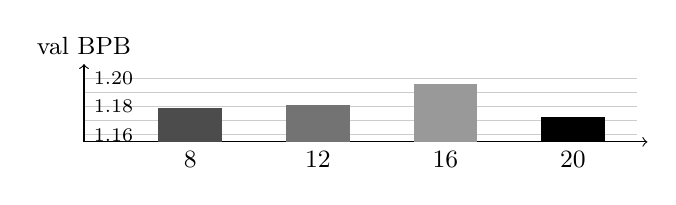
\begin{tikzpicture}[x=1.35cm,y=18cm]
\draw[gray!40] (0,1.16) -- (5.2,1.16);
\draw[gray!40] (0,1.17) -- (5.2,1.17);
\draw[gray!40] (0,1.18) -- (5.2,1.18);
\draw[gray!40] (0,1.19) -- (5.2,1.19);
\draw[gray!40] (0,1.20) -- (5.2,1.20);
\draw[->] (0,1.155) -- (0,1.21) node[above] {\small val BPB};
\draw[->] (0,1.155) -- (5.3,1.155);
\fill[black!70] (0.7,1.155) rectangle (1.3,1.179135);
\fill[black!55] (1.9,1.155) rectangle (2.5,1.180824);
\fill[black!40] (3.1,1.155) rectangle (3.7,1.195546);
\fill[black] (4.3,1.155) rectangle (4.9,1.172248);
\node[below] at (1.0,1.155) {\small 8};
\node[below] at (2.2,1.155) {\small 12};
\node[below] at (3.4,1.155) {\small 16};
\node[below] at (4.6,1.155) {\small 20};
\node[right] at (0,1.16) {\scriptsize 1.16};
\node[right] at (0,1.18) {\scriptsize 1.18};
\node[right] at (0,1.20) {\scriptsize 1.20};
\end{tikzpicture}
\caption{Validation BPB versus depth at fixed $D_{\mathrm{actual}}$. Axis starts at 1.155 to show the sub-0.03 spread. The visual dip at depth 20 is smaller than the registered 0.01 interpretation threshold. Source: Table~\ref{tab:primary}.}
\label{fig:valbpb}
\end{figure}

$D^{\ast}=20$ by exact numerical minimum. Margin to depth 8 is $0.006887$ BPB; to depth 12 is $0.008576$ BPB. With one seed, those gaps are not a ranking. Depth 20 and depth 8 are practically indistinguishable at the registered threshold.

\subsection{Prediction outcome}
The numerical minimum is at depth 20. The series does not show a clean fall-then-flatten across $8\rightarrow 12\rightarrow 16\rightarrow 20$. Validation BPB rises from 8 to 16, then depth 20 is lowest by a sub-0.01 margin over depth 8. The train--validation gap widens from 8 to 16 ($0.342$ to $0.738$) and is $0.500$ at depth 20. Falsification in the strong form (larger depths keep improving held-out BPB at $D_{3x}$ with no increase in the train--validation gap) did not occur. The study does not claim that deeper is always better.

\subsection{Secondary confirmatory test}
After the sealed validation selection, one test BPB was computed on depth 20 only: $1.164768$. Test SHA-256 \texttt{3bd19345\ldots 93baf}. Test was not used to choose $D^{\ast}$. No test BPB is reported for depths 8, 12, or 16. Confirmatory test-read events equal 1.

\subsection{Required baselines}
All four trained models beat the untrained control ($\approx 3.289$) and the byte unigram ($4.453225$). That answers the registered baseline check. It does not rank depths.

\subsection{Secondary analyses, not used for $D^{\ast}$}
These numbers are retained because the close-out checklist requires them. They are not confirmatory depth rankings.

\begin{itemize}
\item In-training 262{,}144-token card BPB: 1.124545 (d8), 1.125139 (d12), 1.137399 (d16), 1.117213 (d20).
\item Depth 12 mid-run minimum $1.084991$ at step 200 was not selected.
\item $D_{1x}$ pilots (step 98): d8 $1.420188$, d12 $1.428635$, both worse than matching $D_{3x}$ seed-0 validation BPB.
\item Extra seeds 1 and 2 at d8 and d12, validation only: d8 mean $1.190892$ (sample SD $0.010318$); d12 mean $1.187442$ (sample SD $0.008792$). The $0.0069$ d20--d8 gap sits inside that noise scale.
\item Document-level non-overlapping bootstrap (1000 resamples, not BOS-bestfit): all four 95\% intervals overlap (about $1.23$--$1.39$).
\item gzip $-9$ on raw validation UTF-8: $2.739$ bits/byte. A compressor is not a causal language model.
\item Samples from $D^{\ast}$ are Tagalog-Wikipedia-flavored and often incoherent. They are not a metric.
\end{itemize}

Packed \texttt{val\_bpb\_full} scores $5{,}868{,}797$ target bytes ($1{,}286{,}864$ tokens). Raw validation UTF-8 is $6{,}771{,}275$ bytes. The unigram uses the raw stream, as registered.

\section{Discussion}
\label{sec:discussion}

The honest reading is narrow. On this reconstructed WikiText-TL-39 package, at $D_{3x}$ and one seed, making nanochat deeper from 8 to 20 does not produce a validation-BPB gap that clears the study's own $0.01$ rule. The train--validation gap does widen as depth increases from 8 to 16, which matches one branch of the registered prediction and is consistent with data-constrained scaling~\cite{hoffmann2022chinchilla,muennighoff2023dataconstrained}. Depth 20 then shows a smaller gap than depth 16 and a slightly lower validation BPB than depth 8. That pattern is a one-seed observation, not a law.

$R_d$ at depth 20 is $0.044$. A Chinchilla-style reading would say the larger models are starved of unique tokens~\cite{hoffmann2022chinchilla}. The study did not skip those depths, because the grid was filed in advance. Skipping them after seeing BPB would have been a protocol break.

The reconstructed split is a limitation that must stay in the caption. Claiming the original 2019 Cruz--Cheng files would be false~\cite{cruz2019eval}. Article reconstruction ($120{,}971$ versus the 2019 table's $120{,}975$) was close enough to keep the article unit. Moses-token counts on this mirror are lower than the 2019 table. The package is the registered Parquet file, not a byte-identical 2019 dump.

Cheng-group papers from 2023--2026 typically report a task score on a constructed Philippine dataset and stop~\cite{espiritu2023balarila,vicente2024vardial,ong2025aigenerated}. This paper does the same for language-modeling BPB. It does not convert a $0.0069$ dip into a general statement about Filipino, chat quality, or English transfer.

\section{Limitations}
\label{sec:limits}

\begin{itemize}
\item Original 2019 splits were not recovered.
\item One seed for the four-depth comparison.
\item WikiText-TL-39 is 2019 Tagalog Wikipedia, not general Filipino web text and not code-switched Taglish~\cite{cruz2019eval}.
\item BOS-bestfit packing crops long documents. Packed target bytes are 13.3\% below raw validation UTF-8.
\item Twenty-nine long articles were newline-chunked for shards. Official $T_{\mathrm{train}}$ is full-article encode.
\item FlashAttention versus SDPA can change numerics across hosts. Confirmatory numbers are from the named A40.
\item No chat, SFT, instruction following, CORE, or classification.
\item Native-speaker ratings do not exist.
\item Extra-seed and $D_{1x}$ files may remain only on a stopped pod volume. Confirmatory weights and logs are on the author's archive and on Hugging Face.
\end{itemize}

\section{Future research}
\label{sec:future}

The following items are exploratory unless a new registration says otherwise.

\begin{enumerate}
\item More seeds on the same frozen $D_{3x}$ grid, validation only, to test whether the $0.0069$ gap is stable. Extra-seed SDs already suggest it may not be.
\item A separately labeled $D_{10x}$ or native-ratio family. Those runs see the corpus more often and are not this experiment~\cite{muennighoff2023dataconstrained}.
\item Recovering or reconstructing a closer match to the 2019 files, if a verified archive appears.
\item Measuring crop rate and document-length effects under BOS-bestfit versus per-document packing.
\item Train-only tokenizer ablations (vocabulary size, byte fallback) that do not leak validation text.
\item Downstream Philippine tasks from the Cheng-group line (grammar correction, NER, authorship, Chavacano) as transfer probes, not as replacements for BPB~\cite{espiritu2023balarila,chan2023ner,espiritu2024aa,vicente2026chavacano}.
\item Larger unique Tagalog corpora (TLUnified-scale or later) with the same equal-exposure discipline~\cite{cruz2022tlunified}.
\item Chat SFT and CORE, only as named follow-ons.
\end{enumerate}

\section{Conclusion}
\label{sec:conclusion}

This paper reported a preregistered, equal-exposure depth sweep of nanochat on WikiText-TL-39. The original 2019 splits were not recovered. The study used a documented article-hash reconstruction, a train-only 32{,}768 BPE tokenizer, and a common $19.27$ million token budget. Depth 20 had the lowest final validation BPB ($1.172248$). The margin to depth 8 was $0.006887$ BPB. Under the registered one-seed rule, that is not a depth ranking. The train--validation gap widened from depth 8 to 16. One test BPB was read after selection. All four models beat untrained and byte-unigram controls.

The original contribution is the locked measurement: same tokens, same tokenizer, same split, four depths, one test touch, and a refusal to promote a sub-0.01 gap. The paper does not claim a general Filipino foundation model, a chat system, or that deeper is always better.

\section*{Novelty statement}
The paper advances Tagalog language-modeling evidence by replacing an informal ``train a deeper nanochat'' demonstration with a preregistered equal-exposure comparison on a public Wikipedia-style corpus. It records a recoverable split after the 2019 files disappeared from the public mirror, and it separates confirmatory BPB from diagnostic curves, extra seeds, and samples. The empirical advance is negative at the study's own threshold: depth is not a ranking factor on this budget and seed.

\section*{Data, code, and weights}
Parquet source: \texttt{linkanjarad/Wikitext-TL39}. Registration: AsPredicted \#306780. Evaluator and manifests: study repository. Seed-0 checkpoints: \texttt{d20/}, \texttt{d16/}, \texttt{d12/}, \texttt{d8/} at \url{https://huggingface.co/pageman/nanochat-filipino-p1-fixed-d20-3x}. Held-out \texttt{test.jsonl} is not redistributed in public zips. ResearchBox \#8735 is the preregistration deposit box.

\section*{Ethics}
The corpus is public Wikipedia-derived text. No human-subjects experiment was run. Sample ratings were not fabricated. Secrets (host credentials, box passcodes) are not published with this paper.

\section*{Acknowledgements}
WikiText-TL-39 is due to Cruz and Cheng~\cite{cruz2019eval}. nanochat is due to Karpathy~\cite{karpathy2026nanochat}. Cheng is not a coauthor of this study. Errors are the author's.

\section*{Funding}
No external grant funded the confirmatory runs. Official training used a rented A40.

\begin{thebibliography}{99}

\bibitem{cruz2019eval}
J.~C.~B. Cruz and C.~Cheng.
\newblock Evaluating language model finetuning techniques for low-resource languages.
\newblock \emph{arXiv:1907.00409}, 2019.

\bibitem{merity2017pointer}
S.~Merity, C.~Xiong, J.~Bradbury, and R.~Socher.
\newblock Pointer sentinel mixture models.
\newblock In \emph{International Conference on Learning Representations}, 2017.

\bibitem{cruz2022tlunified}
J.~C.~B. Cruz and C.~Cheng.
\newblock Improving large-scale language models and resources for Filipino.
\newblock In \emph{Proceedings of the Thirteenth Language Resources and Evaluation Conference}, pages 6548--6555, Marseille, 2022.

\bibitem{cruz2020fakenews}
J.~C.~B. Cruz, J.~A. Tan, and C.~Cheng.
\newblock Localization of fake news detection via multitask transfer learning.
\newblock In \emph{Proceedings of the Twelfth Language Resources and Evaluation Conference}, pages 2596--2604, 2020.

\bibitem{vaswani2017attention}
A.~Vaswani, N.~Shazeer, N.~Parmar, J.~Uszkoreit, L.~Jones, A.~N. Gomez, {\L}.~Kaiser, and I.~Polosukhin.
\newblock Attention is all you need.
\newblock In \emph{Advances in Neural Information Processing Systems}, 2017.

\bibitem{kaplan2020scaling}
J.~Kaplan, S.~McCandlish, T.~Henighan, T.~B. Brown, B.~Chess, R.~Child, S.~Gray, A.~Radford, J.~Wu, and D.~Amodei.
\newblock Scaling laws for neural language models.
\newblock \emph{arXiv:2001.08361}, 2020.

\bibitem{henighan2020scaling}
T.~Henighan, J.~Kaplan, M.~Katz, M.~Chen, C.~Hesse, J.~Jackson, H.~Jun, T.~B. Brown, P.~Dhariwal, S.~Gray, C.~Hallacy, B.~Mann, A.~Radford, A.~Ramesh, N.~Ryder, D.~M. Ziegler, J.~Schulman, D.~Amodei, and S.~McCandlish.
\newblock Scaling laws for autoregressive generative modeling.
\newblock \emph{arXiv:2010.14701}, 2020.

\bibitem{hoffmann2022chinchilla}
J.~Hoffmann, S.~Borgeaud, A.~Mensch, E.~Buchatskaya, T.~Cai, E.~Rutherford, D.~de~Las~Casas, L.~A. Hendricks, J.~Welbl, A.~Clark, T.~Hennigan, E.~Noland, K.~Millican, G.~van~den Driessche, B.~Damoc, A.~Guy, S.~Osindero, K.~Simonyan, E.~Elsen, J.~W. Rae, O.~Vinyals, and L.~Sifre.
\newblock Training compute-optimal large language models.
\newblock \emph{arXiv:2203.15556}, 2022.

\bibitem{muennighoff2023dataconstrained}
N.~Muennighoff, A.~Rush, B.~Barak, T.~L. Scao, N.~Tazi, A.~Piktus, S.~Pyysalo, T.~Wolf, and C.~A. Raffel.
\newblock Scaling data-constrained language models.
\newblock In \emph{Advances in Neural Information Processing Systems}, 2023.

\bibitem{biderman2023pythia}
S.~Biderman, H.~Schoelkopf, Q.~G. Anthony, H.~Bradley, K.~O'Brien, E.~Hallahan, M.~A. Khan, S.~Purohit, U.~S. Prashanth, E.~Raff, A.~Skowron, L.~Sutawika, and O.~van~der Wal.
\newblock Pythia: A suite for analyzing large language models across training and scaling.
\newblock In \emph{Proceedings of the 40th International Conference on Machine Learning}, 2023.

\bibitem{brown2020gpt3}
T.~B. Brown, B.~Mann, N.~Ryder, M.~Subbiah, J.~Kaplan, P.~Dhariwal, A.~Neelakantan, P.~Shyam, G.~Sastry, A.~Askell, S.~Agarwal, A.~Herbert-Voss, G.~Krueger, T.~Henighan, R.~Child, A.~Ramesh, D.~M. Ziegler, J.~Wu, C.~Winter, C.~Hesse, M.~Chen, E.~Sigler, M.~Litwin, S.~Gray, B.~Chess, J.~Clark, C.~Berner, S.~McCandlish, A.~Radford, I.~Sutskever, and D.~Amodei.
\newblock Language models are few-shot learners.
\newblock In \emph{Advances in Neural Information Processing Systems}, 2020.

\bibitem{radford2019gpt2}
A.~Radford, J.~Wu, R.~Child, D.~Luan, D.~Amodei, and I.~Sutskever.
\newblock Language models are unsupervised multitask learners.
\newblock OpenAI technical report, 2019.

\bibitem{sennrich2016bpe}
R.~Sennrich, B.~Haddow, and A.~Birch.
\newblock Neural machine translation of rare words with subword units.
\newblock In \emph{Proceedings of the 54th Annual Meeting of the Association for Computational Linguistics}, pages 1715--1725, 2016.

\bibitem{kudo2018sentencepiece}
T.~Kudo and J.~Richardson.
\newblock SentencePiece: A simple and language independent subword tokenizer and detokenizer for neural text processing.
\newblock In \emph{Proceedings of the 2018 Conference on Empirical Methods in Natural Language Processing: System Demonstrations}, pages 66--71, 2018.

\bibitem{gao2020pile}
L.~Gao, S.~Biderman, S.~Black, L.~Golding, T.~Hoppe, C.~Foster, J.~Phang, H.~He, A.~Thite, N.~Nabeshima, S.~Presser, and C.~Leahy.
\newblock The Pile: An 800GB dataset of diverse text for language modeling.
\newblock \emph{arXiv:2101.00027}, 2020.

\bibitem{shannon1951prediction}
C.~E. Shannon.
\newblock Prediction and entropy of printed English.
\newblock \emph{Bell System Technical Journal}, 30(1):50--64, 1951.

\bibitem{graves2013generating}
A.~Graves.
\newblock Generating sequences with recurrent neural networks.
\newblock \emph{arXiv:1308.0850}, 2013.

\bibitem{melis2018eval}
G.~Melis, C.~Dyer, and P.~Blunsom.
\newblock On the state of the art of evaluation in neural language models.
\newblock In \emph{International Conference on Learning Representations}, 2018.

\bibitem{levine2020depth}
Y.~Levine, N.~Wies, O.~Sharir, H.~Bata, and A.~Shashua.
\newblock The depth-to-width interplay in self-attention.
\newblock In \emph{Advances in Neural Information Processing Systems}, 2020.

\bibitem{press2020reordering}
O.~Press, N.~A. Smith, and O.~Levy.
\newblock Improving transformer models by reordering their sublayers.
\newblock In \emph{Proceedings of the 58th Annual Meeting of the Association for Computational Linguistics}, pages 2996--3005, 2020.

\bibitem{tay2022scale}
Y.~Tay, M.~Dehghani, J.~Rao, W.~Fedus, S.~Abnar, H.~W. Chung, S.~Narang, D.~Yogatama, A.~Vaswani, and D.~Metzler.
\newblock Scale efficiently: Insights from pre-training and fine-tuning transformers.
\newblock In \emph{International Conference on Learning Representations}, 2022.

\bibitem{conneau2020xlmr}
A.~Conneau, K.~Khandelwal, N.~Goyal, V.~Chaudhary, G.~Wenzek, F.~Guzm{\'a}n, E.~Grave, M.~Ott, L.~Zettlemoyer, and V.~Stoyanov.
\newblock Unsupervised cross-lingual representation learning at scale.
\newblock In \emph{Proceedings of the 58th Annual Meeting of the Association for Computational Linguistics}, pages 8440--8451, 2020.

\bibitem{cahyawijaya2023nusacrowd}
S.~Cahyawijaya, H.~Lovenia, A.~F. Aji, G.~I. Winata, B.~Wilie, R.~Mahendra, C.~Wibowo, A.~Romiadhon, Y.~Lovenia, and P.~Fung.
\newblock NusaCrowd: Open source initiative for Indonesian NLP resources.
\newblock In \emph{Findings of the Association for Computational Linguistics: ACL 2023}, 2023.

\bibitem{espiritu2023balarila}
P.~Espiritu, J.~Jadie, A.~Ponce, and C.~Cheng.
\newblock Balarila: Deep learning for semantic grammar error correction in low-resource settings.
\newblock In \emph{Proceedings of the First Workshop in South East Asian Language Processing}, 2023.

\bibitem{velasco2023wordnet}
D.~J. Velasco, A.~Alba, T.~G. Pelagio, B.~A. Ramirez, J.~C.~B. Cruz, U.~Chua, B.~P. Samson, and C.~Cheng.
\newblock Towards automatic construction of Filipino WordNet: Word sense induction and synset induction using sentence embeddings.
\newblock In \emph{Proceedings of the First Workshop in South East Asian Language Processing}, 2023.

\bibitem{chan2023ner}
K.~Chan, K.~A. De~Las~Alas, C.~Orcena, D.~J. Velasco, Q.~J. San~Juan, and C.~Cheng.
\newblock Practical approaches for low-resource named entity recognition of Filipino telecommunications domain.
\newblock In \emph{Proceedings of the 37th Pacific Asia Conference on Language, Information and Computation}, 2023.

\bibitem{vicente2024vardial}
A.~J. Vicente and C.~Cheng.
\newblock Language identification of Philippine Creole Spanish: Discriminating Chavacano from related languages.
\newblock In \emph{Proceedings of the Eleventh Workshop on NLP for Similar Languages, Varieties and Dialects}, 2024.

\bibitem{espiritu2024aa}
P.~Espiritu, J.~Jabanes, and C.~Cheng.
\newblock Authorship attribution in 19th-century Philippine literature using a deep learning multi-label classifier.
\newblock In \emph{Proceedings of the 38th Pacific Asia Conference on Language, Information and Computation}, 2024.

\bibitem{loquinte2024formality}
K.~U. Loquinte and C.~Cheng.
\newblock Modified iterative matching and translation approach for formality style transfer in a low-resource setting.
\newblock In \emph{Proceedings of the 38th Pacific Asia Conference on Language, Information and Computation}, 2024.

\bibitem{ong2025aigenerated}
C.~Ong and C.~Cheng.
\newblock Detecting AI-generated Filipino text: A synthetic data approach with pre-trained LLMs.
\newblock In \emph{2025 International Conference on Asian Language Processing (IALP)}, pages 42--47, 2025.

\bibitem{marcellana2025sarcasm}
P.~J. Marcellana and C.~Cheng.
\newblock Leveraging synthetic data and LLMs for sarcasm detection.
\newblock In \emph{2025 International Conference on Asian Language Processing (IALP)}, 2025.

\bibitem{tahimic2025sae}
K.~Tahimic and C.~Cheng.
\newblock Mechanistic interpretability of code correctness in LLMs via sparse autoencoders.
\newblock \emph{arXiv:2510.02917}, 2025.

\bibitem{vicente2026chavacano}
A.~J. Vicente, T.~F. Amamampang, D.~D. Lahaylahay, and C.~Cheng.
\newblock ChavacanoMT: A corpus and evaluation of neural machine translation for Philippine Creole Spanish.
\newblock \emph{Language Resources and Evaluation}, 2026.

\bibitem{nosek2018prereg}
B.~A. Nosek, C.~R. Ebersole, A.~C. DeHaven, and D.~T. Mellor.
\newblock The preregistration revolution.
\newblock \emph{Proceedings of the National Academy of Sciences}, 115(11):2600--2606, 2018.

\bibitem{simmons2011falsepositive}
J.~P. Simmons, L.~D. Nelson, and U.~Simonsohn.
\newblock False-positive psychology: Undisclosed flexibility in data collection and analysis allows presenting anything as significant.
\newblock \emph{Psychological Science}, 22(11):1359--1366, 2011.

\bibitem{wagenmakers2012confirmatory}
E.-J. Wagenmakers, R.~Wetzels, D.~Borsboom, H.~L. van~der Maas, and R.~Kievit.
\newblock An agenda for purely confirmatory research.
\newblock \emph{Perspectives on Psychological Science}, 7(6):632--638, 2012.

\bibitem{munafo2017manifesto}
M.~R. Munafo, B.~A. Nosek, D.~V. Bishop, K.~S. Button, C.~D. Chambers, N.~Percie~du Sert, U.~Simonsohn, E.-J. Wagenmakers, J.~J. Ware, and J.~P.~A. Ioannidis.
\newblock A manifesto for reproducible science.
\newblock \emph{Nature Human Behaviour}, 1:0021, 2017.

\bibitem{aspredicted306780}
P.~Pajo.
\newblock NANOCHAT-FILIPINO P1.1: WikiText-TL-39 fixed-budget depth vs held-out BPB.
\newblock AsPredicted \#306780, 15 August 2026.
\newblock \url{https://aspredicted.org/6r6v4v.pdf}.

\bibitem{karpathy2026nanochat}
A.~Karpathy.
\newblock nanochat.
\newblock Software repository, 2026.
\newblock \url{https://github.com/karpathy/nanochat}.

\end{thebibliography}

\end{document}
